\documentclass[letterpaper,11pt]{article}

\usepackage[margin=1in]{geometry}
\usepackage{times}
\usepackage[compact]{titlesec}
\usepackage{amsmath,amssymb,amsthm}
\usepackage{graphicx}
\usepackage{subcaption}
\usepackage{hyperref}
\usepackage[T1]{fontenc}
\usepackage[giveninits=true]{biblatex}
%\usepackage[style=mla]{biblatex}
\usepackage{tabularx}
\usepackage{cleveref}
\usepackage{tikz}

\usetikzlibrary{arrows.meta}
\usetikzlibrary{shapes.geometric}
\usetikzlibrary{shapes.multipart}
\usetikzlibrary{cd}

\addbibresource{ref23.bib}

\graphicspath{
    {Figs/},{figures/}
}

\titleformat*{\paragraph}{\itshape}

\newcommand{\cF}{{\mathcal{F}}}
\newcommand{\cX}{{\mathcal{X}}}

\begin{document}

\thispagestyle{empty}
\noindent\textbf{ANNUAL REPORT}\\[1cm]
\centerline{\textbf{\Large Unified Large-Scale Theoretical and Computational Frameworks}}
\centerline{\textbf{\Large for Invariance and Composition of Open Hybrid Dynamical Systems}}\\[1cm]

\renewcommand\arraystretch{1.5}
\begin{tabularx}{1.0\textwidth}{>{\bfseries}lX}
Award Number & FA9550-23-1-0400\\
Report Type & Annual\\
Reporting Period & July 2, 2023 - July 1, 2024\\
Distribution Statement & Distribution A - Approved for public release\\
Program Officer Name & Dr. Frederick Leve\\
Principal Investigator Name & Dr. Taeyoung Lee\\
Project Title & Unified Large-Scale Theoretical and Computational Frameworks for Invariance and Composition of Open Hybrid Dynamical Systems\\
%
Abstract & This project is to establish both theoretical and computational frameworks to analyze and certify the intriguing behaviors of complicated open hybrid dynamical systems. 
In particular, the objective is to identify and construct the inherent structures of hybrid dynamics, such as topological properties and invariances, that can be preserved under the interaction with uncertain environments and composition over a complex network. 
During YR1, we investigated 15 topics in the area of geometry, topology, openness, scalability, and category of hybrid systems. 
\end{tabularx}

\clearpage\newpage

\tableofcontents

\clearpage\newpage
\setcounter{page}{1}
\section{Research Objectives}
This project will develop theoretical and computational frameworks to analyze and certify the behavior of complex open hybrid dynamical systems, such as embodied artificial intelligence,  quantum systems, and biological systems. 
The objective is to identify and construct the inherent structures of hybrid dynamics, such as topological properties and invariances, that can be preserved under the interaction with an uncertain environment and composition over a complex network.
The novelty lies in establishing a trustworthy computational foundation that is carefully constructed in conjunction with the underlying geometry, leading to a significant generalization capacity and computational efficiency in understanding the global topological properties of complex, composable hybrid systems. 

This will be achieved by multidisciplinary collaborative efforts in dynamical systems and theoretical computer science. 
In particular, we focus on three research thrusts: discovery of geometric and topological structures; investigation of the uncovered structures in open, uncertain environments and composition; extension to gene regulatory networks/multi-agent systems and further generalization to scalable composition and certification, as illustrated in \Cref{fig:overview}.

\usetikzlibrary{matrix, positioning, fit, backgrounds}
\begin{figure}[h]
    \scriptsize
    \centerline{
        \begin{tikzpicture}[
            mymatrix/.style={matrix of nodes, nodes=typetag, row sep=7pt, align = center},
            typetag/.style={draw, thick, fill=white, inner sep=1.5ex, anchor=west, text width = 0.27\textwidth, align = center},
            mycontainer/.style={draw=gray, inner sep=1ex},
            title/.style={draw=none, fill=none, inner sep=0pt, align=center, font=\bfseries},
            analytic/.style={draw},
            mixed/.style={draw, dash dot},
            comp/.style={draw, dotted}
            ]
            \matrix[mymatrix] (GT) {
                |[title]| (i) Geometry \& Topology\\
                |[analytic]| {Geometry and Topology\\ (Bloch, Clark)} \\
                |[mixed]| {Homological Dynamics\\ (Mischaikow, Kalies)} \\
                |[comp]| { Topological Dynamics Learning\\ (Ghaffari, Bloch, Clark) }\\ 
            };
            \matrix[mymatrix, right=20pt of GT.north east, matrix anchor=north west] (OS) {
                |[title]| (ii) Openness \& Scalability\\
                |[analytic]| { Geometry and Topology\\ (Bloch, Clark)} \\
                |[mixed]| { Stochastic Hybrid Network\\ (Lee, Mischaikow, Kalies)} \\
                |[analytic]| { Unified Composition Framework \\ (Guralnik, Vasudevan, Ghaffari) }\\ 
            };
            \matrix[mymatrix, right=20pt of OS.north east, matrix anchor=north west, row sep=5pt] (EV) {
                |[title]| (iii) Extension \& Verification\\
                |[mixed, inner sep=3pt]| { Gene Regulatory Networks\\[-0.05cm] (Mischaikow, Kalies)} \\
                |[mixed, inner sep=3pt]| { Cooperative Multi-agent Systems\\[-0.05cm] (Lee, Guralnik)} \\
                |[comp, inner sep=3pt]|{ Scalable Composition\\[-0.05cm] (Vasudevan, Ghaffari, Guralnik)} \\
                |[comp, inner sep=3pt]| { Formal Verification\\[-0.05cm] (Vasudevan, Lee, Mischaikow) }\\ 
            };
            \node[mycontainer, fit=(GT)] (GTBox) {};%, label={[text width=0.27\textwidth] below:discover topological properties with three distinct approraches}] (GTBox) {};
            \node[mycontainer, fit=(OS)] (OSBox) {};
            \node[mycontainer, fit=(EV)] (EVBox){};

            \begin{scope}[on background layer]
                \node[mycontainer, fit=(GTBox), fill=gray!10, inner sep = 0pt] {};
                \node[mycontainer, fit=(OSBox), fill=gray!10, inner sep = 0pt] {};
                \node[mycontainer, fit=(EVBox), fill=gray!10, inner sep = 0pt] {};
            \end{scope}

            \draw[arrows={-Triangle[angle=30:6pt]}, thick] (GTBox) -- (OSBox);
            \draw[arrows={-Triangle[angle=30:6pt]}, thick] (OSBox) -- (EVBox);
            \draw[arrows={-Triangle[angle=30:6pt]}, thick] (EVBox.south) -- ++(0,-8pt) -- ([yshift=-8pt]GTBox.south) -- (GTBox.south);
        \end{tikzpicture}
    }
    \DeclareRobustCommand\captionsolid{\tikz[baseline=-0.6ex]\draw[thick] (0,0)--(0.5,0);}
    \DeclareRobustCommand\captiondashdot{\tikz[baseline=-0.6ex]\draw[thick, dash dot] (0,0)--(0.5,0);}
    \DeclareRobustCommand\captiondotted{\tikz[baseline=-0.6ex]\draw[thick, dotted] (0,0)--(0.5,0);}
    \caption{Proposed research: (i) we will discover geometric and topological properties of hybrid systems with three distinct approaches: theoretical analysis (\captionsolid), mixed theoretical analysis and computation (\captiondashdot), and computation (\captiondotted); (ii) next, we will investigate how such topological properties are affected by environments, uncertainties, and large-scale compositions; (iii) these will be further extended to gene regulatory networks and multi-agent systems, and they will be verified with formal methods.}\label{fig:overview}
\end{figure}

\newpage

\begin{itemize}
    \item Q: is there any topic that is missing here?
    \item Q: is there any topic with missing names?
    \item Q: is it going to be presented at the MURI review meeting?
    \item Q: it is mature enough to be described as an outcome of YR2, or a direction for YR3, or better not mention yet?
\end{itemize}

\section{Geometry and Topology}
\paragraph*{Outcome}
\subsection{Linear affine hybrid system (Will)}
\subsection{Hybrid Conley index theory (Bill)}
\subsection{Data-driven learning for hybrid systems (Konstantin, Will)}
\subsection{Homological dynamics of hybrid system (Konstantin, Dan)}
\paragraph*{Future Directions}
\subsection{? Data-driven learning for open hybrid system (Tony, Maani)}
\subsection{? HJB + Zeno (Ram,Will …)}
\subsection{? Mechanics and control with collision (Tony, Will)}
\subsection{? Hybrid Holonomy (Dan, Will}
\vspace*{0.3cm}

\section{Openness and Composition}
\paragraph*{Outcome}
\subsection{Hybrid dynamic networks (Tony)}
\subsection{Stochastic hybrid system (Lee, Will)}
\subsection{Geometric numerical integration of stochastic hybrid system (Lee)}
\paragraph*{Future Directions}
\subsection{? Geometric modeling of deterministic state uncertainty (Dan, Lee)}
\subsection{? Hybrid dynamic network for DSGRN (Tony, Konstantin, Bill, Dan)}
\vspace*{0.3cm}


\section{Scalability and Verification}
\paragraph*{Outcome}
\subsection{Hybrid optimal control with affine geometric heat flow (Ram)}
\subsection{Hybrid mean field game (Lee)}
\subsection{DHAL: Discrete hybrid automata learning (Maani, Konstantin, Bill, Will)}
\paragraph*{Future Directions}
%\subsection{? Hybrid, non-holonomic optimal control (Tony)}
\subsection{? Hybrid rigid body optimal control (Maani, Ram, Lee)}
\subsection{? Generalized DSGRN with control (Dan, Konstantin, Bill)}
\subsection{? Invariant filtering for hybrid dynamic network (Lee, Maani)}


\end{document}

\subsection{Scalable Composition for Hybrid Mechanical System Identification (Vasudevan)} 

\paragraph{Research Objectives} System identification for robotic systems interacting with the environment is essential for applications including controller synthesis, model analysis, and observer design. 
However, traditional system identification methods primarily target unconstrained systems, leaving a significant gap in handling robots with closed kinematic chains or other kinds of constraints such as those that arise due to contact with the environment. 
Notably these techniques formulate the identification of model parameters such as inertia and friction as nonlinear programs that can be difficult to solve for high-dimensional robots. 
The goal of this task is to solve the system identification problem for constrained robotic systems in a numerically tractable fashion.

\paragraph{Accomplishments} Typically system identification for robotic systems to identify inertial parameters can be accomplished by performing linear least squares. 
Though this method is powerful it is unable to ensure the physical viability of estimated parameters (e.g., the mass estimate may be negative). 
To address this shortcoming and deal with constraints, during this past year we have developed a linear-matrix inequality method to estimate friction and inertial properties for systems with constraints. 
Typically these LMI approaches can suffer from poor computational scaling which can make applying these techniques to systems with a large number of parameters non-trivial. 
To address these issues, we have shown that one can leverage the branched description of robot dynamics to represent the system identification LMI problem as a much more tractable semidefinite program.
In particular, the semidefinite matrices are block diagonal. 

We have illustrated the utility of this approach by applying it to perform system identification for the 20 degree of freedom humanoid, Digit. 
Notably, each of Digit's legs includes a pair of closed loop kinematic constraints.
During real-world evaluation, we have shown that we can identify inertial and friction parameters that are orders of magnitude more accurate than the one's provided by the manufacturers when applied to predict the behavior of the system.
In addition, we have shown that when these parameters can be applied in the real-world during feedback control to perform much tighter tracking than would have been possible with the parameters provided by the manufacturer. 
Note all experiments conducted thus far have suspended the robot in the air rather than have it interact with the ground.

\paragraph{Plan} Our goal over the coming year is to apply the proposed approach to identify a model of contact that arises when the system interacts with the environment. 
This will not require a drastic reformulation of the method, but will initially rely upon segmenting the data by hand. 
We will then explore how to formulate the optimization problem to automatically segment the data. 
In parallel, we will explore how to compute trajectories that are most informative while performing system identification. 


\subsection{Geometric Integration for Stochastic Mechanical Hybrid System (Lee)}

\paragraph{Research Objectives}

Here we consider stochastic hybrid systems that arise from Lagrangian or Hamiltonian systems undergoing collisions. 
The focus is to develop geometric numerical integration schemes that preserve the underlying structure of the dynamics for long-term stability and robustness in numerical simulations. 
Multiple formulations of stochastic Hamiltonian systems have been presented. It is shown that they can be obtained by extremizing a stochastic action integral. Using this, symplectic numerical methods, referred to as stochastic variational integrators, have been constructed through the discretization of Hamilton’s principle. 
For instance, they have been applied to large dissipative systems with applications to the compressible Navier-Stokes equations.
We extend this idea of structure preserving stochastic variational integrators for the class of hybrid mechanical systems with impact. 

\paragraph{Accomplishments}

This is a challenging problem since discontinuities are introduced in the motion of the system along with the addition of perturbations.
Firstly, we obtain the Euler-Lagrange equations in the continuous-time setting, by utilizing the variational principle for the dynamics with additive noise that is incorporated through a stochastic potential term. 
Next, we adopt the Hamilton-Pontryagin principle to formulate Hamilton’s equations by the variational principle on the Pontryagin bundle. 
These are discretized to obtain structure-preserving variational integrators for the presented stochastic mechanical hybrid systems in both formulations. 
Finally, these are verified by numerical simulations to demonstrate the effectiveness of the constructed integrators. 
It is shown that the proposed methods accurately capture the long-term energy behavior of a stochastic mechanical hybrid system. 

\paragraph{Plan}

This will further extended to stochastic mechanical hybrid systems on manifolds. 
In particular, we intend to investigate the notion of retraction maps, which have been generalized to discretization maps recently~\cite{diego24}. 
Discretization maps can be used to systematically derive numerical integrators that preserve the symplectic structure, as well as the discrete momemtum map under the assumption of symmetric preservation for the discretization map. 
This provides a geometrical construction that can be easily adapted to discretize dynamics on more general structures and open the door to reduction processes.


\section{Extension and Verification}


\subsection{Identifying Catastrophies Relevant to Controllability 
(Kalies, Mischaikow)}\label{sec:catastrophies}

\paragraph{Research Objectives}
The code Dynamic Signatures Generated by Regulatory Networks (DSGRN) \cite{DSGRN} computes dynamics of regulatory networks. It takes a regulatory network as input and produces an explicit subdivision of parameter space where each region of the subdivision is given by an explicit semi-algebraic set \cite{cummins:gedeon:harker:mischaikow:mok,kepley:mischaikow:zhang}. This information is encoded in the \emph{parameter graph}, where each node of the parameter graph represents a region of parameter space and an edge between nodes indicates that the corresponding regions share a codimension-1 hypersurface. The parameter graph for the network in Figure~\ref{fig:wall_labeling}(b) has $1,600$ nodes. For each node of the parameter graph DSGRN computes the dynamics of the network which is valid for all parameters in the corresponding parameter region of parameter space.

The classical DSGRN computes a combinatorial description of dynamics as follows. Given a regulatory network with $N$ nodes, DSGRN creates an abstract $N$-dimensional cell complex $\cX$ representing a decomposition of phase space and defines a multivalued map (directed graph) $\cF$ mapping cells of $\cX^{(N)}$ (the set of $N$-dimensional cells of $\cX$) to sets of cells of $\cX^{(N)}$ describing the local dynamics of the system. Graph algorithms are then used to decompose the set of $N$-dimensional cells of $\cX$ into cells corresponding to recurrent dynamics (nontrivial strongly connected components of $\cF$) and gradient like dynamics. This information in encoded in the \emph{Morse graph}, where the nodes of the Morse graph correspond to collections of cells exhibiting recurrent dynamics and the edges correspond to gradient like dynamics.

The classical DSGRN is a powerful tool to compute dynamics of networks because it is very computationally efficient and it computes the dynamics of a network for the whole parameter space. However there two main drawbacks: (1) Due to the fact that $\cF$ is defined only in terms of the top-dimensional cells of $\cX$, DSGRN computes a coarse description of dynamics; (2) The combinatorial descriptions of dynamics computed by DSGRN is not validated.

As part of our current efforts we produced an new version of DSGRN that addresses these drawbacks by: (1) We include the lower dimensional cells of $\cX$ in the definition of $\cF$ and hence we get a finer description of dynamics; (2) We validate the computed dynamics via the Conley index and prove that the computed dynamics is valid for parameterized families of ODEs defined in terms of the input network.

We define the map $\cF$ in the updated DSGRN as follows. The information from the classical DSGRN is used to represent a discrete flow on the cell complex $\cX$ which is encoded by a \emph{wall labeling}. A wall labeling is a function which assigns $1$ or $-1$ to each \emph{wall} of $\cX$, where walls are defined as a pairs of cells $(\xi, \xi') \in \cX^{(N - 1)} \times \cX^{(N)}$ with $\xi$ a face of $\xi'$. The value of the wall labeling at a wall $(\xi, \xi')$ indicates whether the discrete flow points from the face $\xi$ to the top-dimensional cell $\xi'$ or vice-versa (see Figure~\ref{fig:wall_labeling}(a) for an illustration). This discrete flow defined by the wall labeling is then extended to the lower dimensional cells. Using this extension we have formulas defining a multivalued map $\cF$ which is defined at every cell of $\cX$ (including lower dimensional cells). This map is then used to decompose the cells in $\cX$ into recurrent and gradient-like dynamics and produce a Morse graph as before.

The dynamics computed by this new map $\cF$ is validated using (homological) Conley index. To compute the homology needed for the Conley index we define a \emph{cubical blowup complex} $\cX_b$. The complex $\cX_b$ is defined such that there is a bijection between the top-dimensional cells of $\cX_b$ and the cells of $\cX$. Hence the map $\cF$ defined on $\cX$ can be be identified to a map $\cF$ defined on the top-dimensional cells of $\cX_b$. The homological Conley index is computed via the \emph{connection matrix} using the algorithms in \cite{harker:mischaikow:spendlove}. The connection matrix gives the Conley indices corresponding to each node in the Morse graph and also gives information about connecting orbits between the invariant sets corresponding to these nodes. The Morse graph with the Conley index information associated to each node is called the Conley-Morse graph. Figure~\ref{fig:wall_labeling}(c)-(d) shows the cell complex $\cX_b$, the multi-valued map $\cF$, and the associated Conley-Morse graph corresponding to parameter node $752$ of the network in Figure~\ref{fig:wall_labeling}(b). Code to compute the connection matrix is available at \url{https://github.com/marciogameiro/pyCHomP2}. The dynamics computed is proven to be valid for families of ODEs corresponding to the input regulatory network (this is the subject of a manuscript in preparation).

\begin{figure}[h!]
\begin{picture}(430, 125)(0, 0)
%
\put(0, -5){(a)}
\put(0, 0){
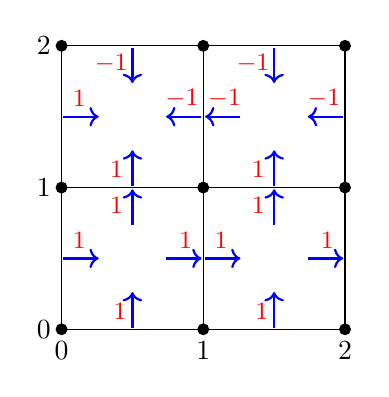
\begin{tikzpicture}[scale=0.225]
% Draw the large grid
\draw[step=8cm, black] (0,0) grid (16,16);
% zero cells
\foreach \i in {0,...,2}{
\foreach \j in {0,...,2}{
\draw[black, fill=black] (8*\i,8*\j) circle (2ex);
} }
% draw grid numbers
\foreach \i in {0,...,2}{
\draw(8*\i, -1.2) node{$\i$}; % row
\draw(-1, 8*\i) node{$\i$}; % column
}
%
% draw wall labelling arrows
\draw[->, blue, thick] (4,          0.1) -- (4,          2.1);
\draw[->, blue, thick] (4 + 8,      0.1) -- (4 + 8,      2.1);
\draw[->, blue, thick] (0.1,          4) -- (2.1,          4);
\draw[->, blue, thick] (8 - 2.1,      4) -- (8 - 0.1,      4);
\draw[->, blue, thick] (8 + 0.1,      4) -- (8 + 2.1,      4);
\draw[->, blue, thick] (16 - 2.1,     4) -- (16 - 0.1,     4);
\draw[->, blue, thick] (4,      8 - 2.1) -- (4,      8 - 0.1);
\draw[->, blue, thick] (4 + 8,  8 - 2.1) -- (4 + 8,  8 - 0.1);
\draw[->, blue, thick] (4,      8 + 0.1) -- (4,      8 + 2.1);
\draw[->, blue, thick] (4 + 8,  8 + 0.1) -- (4 + 8,  8 + 2.1);
\draw[->, blue, thick] (0.1,      8 + 4) -- (2.1,      8 + 4);
\draw[->, blue, thick] (8 - 0.1,  8 + 4) -- (8 - 2.1,  8 + 4);
\draw[->, blue, thick] (8 + 2.1,  8 + 4) -- (8 + 0.1,  8 + 4);
\draw[->, blue, thick] (16 - 0.1, 8 + 4) -- (16 - 2.1, 8 + 4);
\draw[->, blue, thick] (4,     16 - 0.1) -- (4,     16 - 2.1);
\draw[->, blue, thick] (4 + 8, 16 - 0.1) -- (4 + 8, 16 - 2.1);
% draw wall labelling values
\draw[red] (4 - 0.7,          1) node{{\small $1$}};
\draw[red] (4 + 8 - 0.7,      1) node{{\small $1$}};
\draw[red] (1,            4 + 1) node{{\small $1$}};
\draw[red] (8 - 1,         4+ 1) node{{\small $1$}};
\draw[red] (8 + 1,         4+ 1) node{{\small $1$}};
\draw[red] (16 - 1,        4+ 1) node{{\small $1$}};
\draw[red] (4 - 0.9,      8 - 1) node{{\small $1$}};
\draw[red] (4 + 8 - 0.9,  8 - 1) node{{\small $1$}};
\draw[red] (4 - 0.9,      8 + 1) node{{\small $1$}};
\draw[red] (4 + 8 - 0.9,  8 + 1) node{{\small $1$}};
\draw[red] (1,        8 + 4 + 1) node{{\small $1$}};
\draw[red] (8 - 1.2,  8 + 4 + 1) node{{\small $-1$}};
\draw[red] (8 + 1.2,  8 + 4 + 1) node{{\small $-1$}};
\draw[red] (16 - 1.2, 8 + 4 + 1) node{{\small $-1$}};
\draw[red] (4 - 1.2,     16 - 1) node{{\small $-1$}};
\draw[red] (4 + 8 - 1.2, 16 - 1) node{{\small $-1$}};
\end{tikzpicture}
}
%
\put(135, -3){(b)}
\put(130, 10){
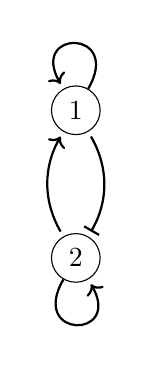
\begin{tikzpicture}
[main node/.style={circle,fill=white!20,draw},scale=2.5]
\node[main node] (1) at (0,0.75) {1};
\node[main node] (2) at (0,0) {2};        
\path[thick]
(1) edge[-|,shorten <= 2pt, shorten >= 2pt, bend left] (2)
(2) edge[loop left, distance=10pt, shorten >= 2pt, thick, in=300, out=240, ->] (2)
(2) edge[->,shorten <= 2pt, shorten >= 2pt, bend left] (1)
(1) edge[loop right, distance=10pt, shorten >= 2pt, thick, in=120, out=60, ->] (1); 
\end{tikzpicture}
}
%
\put(175, -3){(c)}
\put(170, 10){
\includegraphics[width=0.28\textwidth]{figures/stg_2D_saddle_saddle_connection.pdf}
}
%
\put(300, -3){(d)}
\put(280, 0){
\includegraphics[width=0.4\textwidth]{figures/mg_2D_saddle_saddle_connection.pdf}
}
\end{picture}
\caption{(a) Visual representation of a wall labeling; (b) Regulatory network; (c) Representation of the $2$-dimensional cell complex $\cX_b$ and multi-valued map $\cF$ (blue arrows) corresponding to parameter node $572$ of the network in (b); (d) Conley-Morse graph corresponding to parameter node $752$ of the network in (b). Each node in the Conley-Morse graph is annotated with its Conley index represented by their Betti numbers $(\beta_0,\beta_1,\beta_2)$.}
\label{fig:wall_labeling}
\end{figure}


For parameterized families of dynamical systems, attractors have the structure of a sheaf over the parameter space. These attractor sheaves are conjugacy invariants of the parameterized family and algebraically characterize the continuation of sections of attractors over regions in the parameter space, as measured through attracting neighborhoods.  This structure was recently established in \cite{sheaf} and provides an algebraic framework to study bifurcations through sheaf cohomology. 


\paragraph{Accomplishments} As part of the new version of DSGRN we produced the following code (available at \url{https://github.com/marciogameiro/DSGRN} and \url{https://github.com/marciogameiro/DSGRN_utils}). The new DSGRN can compute the dynamics for each node of the parameter graph (and hence for the whole parameter graph). However just computing the dynamics of each node is not convenient when we need to perform multiple queries into the types of dynamics exhibited by the network. For this reason we developed code to organize the information produced by DSGRN into a queryable database which can be queried for different types of dynamics, such as bistability, multistability, stable cycles, etc.

This reporting period we have begun to establish a computational framework to use the theoretical results in \cite{sheaf} to study bifurcations through a cellular sheaf approximation of the attractor sheaf using combinatorial dynamics. This effort has been on two fronts: applications within the DSGRN framework and more generally for combinatorial dynamics.

In the context of DSGRN, where the parameter spaces are high-dimensional but naturally partitioned into cells, across the boundaries of which the Conley-Morse graph changes, a cellular sheaf can be constructed from these parameter cells. The new code to make searchable queries of dynamics across the parameter graph has facilitated  sheaf computations. In particular, we have used attractor sheaves to discover paths in parameter space that exhibit hysteresis, as well as higher-codimension bifurcations, including the cusp bifurcation. These higher-codimension bifurcations are organizing centers in the bifurcation structure. To discover these bifurcations, we first determine the signature in the sheaf structure corresponding to a specific bifurcation and then search through the parameter space for this signature. 

 In the case of the cusp bifurcation, new methods for rigorous computer-assisted verification of cusp bifurcations in low-dimensional parameter spaces has been recently developed \cite{rigorous_cusp}. Preliminary computations suggest that one can detect the signature of a cusp bifurcation in the high-dimensional parameter spaces of DSGRN, determine specific data from the small number of parameter cells involved, and input this data into the verification code to rigorously verify via computer-assisted proof that a cusp bifurcation occurs within a two-dimensional submanifold of the parameter space.

In general, the cellular sheaf determined from combinatorial dynamics are only approximations to the attractor sheaf of the underlying system. However, for certain bifurcations, such as blue sky bifurcations like the saddle-node, the existence of the sheaf signature for the bifurcation and knowledge of the sets involved in the phase space are enough to establish that a bifurcation occurs in the underlying system. 

\paragraph{Plan}  As indicated above the results described in the accomplishments section range from preliminary theoretical results to preliminary computational techniques.
Our immediate plan is to build code that can automatically take in network structures, perform the DSGRN computations, and identify generalized hysteretic switches and cusp bifurcations. 
These tools will be designed with applications involving  regulatory networks arising in systems biology and genetic engineering, and tested against the problem of identifying small networks that exhibit switching over large parameter ranges and identifying the global bifurcation structure of larger networks such as those that control the epithelial mesenchymal transition, where it is speculated that inopportune saddle-node bifucations lead to states that are associated with metastasis, tumor invasion, tissue fibrosis, etc.
We will also consider the problem of identifying higher order catastrophes.


\subsection{Topological Tools for Robotic Control (Mischaikow)}\label{sec:topo tools for control}

\paragraph{Research Objectives}
Our efforts are motivated by two observations. 
First, accuracy (as opposed to precision) is of fundamental concern in robotic control -- it is more important to know that the robot will carry out the task successfully as opposed to having the capability of carrying out the task at arbitrary levels of precision.
Second, the current trend for control of complex systems is based on machine learned controllers.
Conceptually, techniques based on algebraic topological invariants should be able to guarantee results, while only requiring information up to homotopy classes. 
Our objective is to realize this conceptual perspective.

\paragraph{Accomplishments}
Estimating the Region of Attraction (RoA) for a robot controller is crucial for ensuring safe application and effective controller composition. 
Existing methods often necessitate a closed-form expression, limiting their utility for data-driven controllers, or are highly data-intensive when relying solely on trajectory sampling. 
In prior work, topological tools based on Morse Graphs (directed acyclic graphs that combinatorially represent the underlying nonlinear dynamics) have demonstrated data-efficient RoA estimation without requiring an analytical model. 
However, these tools struggle with high-dimensional systems due to the need for state-space discretization. 
The paper \cite{vieira2024morals} (which was a finalist for the best Automation Paper Award) introduces a novel approach, named \textit{Morse Graph-aided discovery of Regions of Attraction in a learned Latent Space} (MoRALS), which leverages auto-encoding neural networks to project high-dimensional dynamics into a lower-dimensional latent space, combined with Morse Graphs to estimate attractors and their RoAs efficiently. The framework discovers an embedding into a low-dimensional latent space, where it can perform its operations using significantly less data. It provides as output a \textit{bistability graph}, an explainable representation of the success and failure regions of the original high-dimensional system. The method is validated on high-dimensional robotic systems, including a 67-dimensional humanoid robot and a 96-dimensional 3-fingered manipulator, demonstrating significant data efficiency and predictive capability in RoA estimation for data-driven controllers. By projecting the controlled system's dynamics into a latent space, MoRALS constructs a reduced Morse Graph that identifies bistability in the system's dynamics, distinguishing between desired and undesired behaviors. The results indicate that MoRALS offers a robust solution for RoA estimation in high-dimensional systems where traditional methods are computationally prohibitive or infeasible, showcasing how rigorous mathematical tools can combine with state-of-the-art machine learning techniques to understand high-dimensional dynamical systems in an explainable manner.

Retrieving a target object from a messy and constrained space, such as taking out a bottle of water from a fridge, requires a robotic arm to relocate other objects blocking access. Traditional prehensile operations, such as picking and placing objects, can be laborious in dense clutter, prompting the use of non-prehensile actions like pushing multiple objects simultaneously to clear space. However, this introduces uncertainty due to the unpredictable outcomes of pushing. The paper \cite{9811848} presents a novel framework combining topological tools and Monte-Carlo Tree Search (MCTS) to enhance the efficiency and robustness of pushing actions for object retrieval. The proposed method takes advantage of persistent homology to inform the selection of efficient and robust pushing actions, without manual hyper-parameter adjustments. MCTS then explores feasible pushing actions, aiming to minimize operations needed to clear the path to the target object. Real-world experiments with a Baxter robot demonstrate that this approach achieves higher success rates and fewer actions in cluttered environments compared to alternatives, ensuring reliability even with offline planning.

\paragraph{Plan}
While MoRALS provides state of the art capability for identifying the RoA for high dimensional problems, from a purely conceptual perspective it has inherent inefficiency and inaccuracy.
The above mentioned reduced Morse graph arises from a condensation graph of a combinatorial model of the robotic dynamics.
MoRALS computes this condensation graph using the latent dynamics. 
However, conceptually identifying the condensation graph can be viewed as a classification problem of regions of phase space. 
Our goal is to machine learn this classification problem directly, thus eliminating the need for constructing latent dynamics and avoiding errors introduced by the latent dynamics.




\subsection{Category-theoretical Approach to Strategy Spaces (Guralnik)}\label{sec:strategy spaces}
%

\paragraph{Research Objectives}
%
Strategy spaces for finite transition systems $\mathcal{T}$ are a theoretical construction (denoted $\Delta_\mathcal{T})$ introduced by Michael Erdmann to enable the design of non-deterministic and stochastic transition systems with desired controllability properties.
%
A fundamental result states that a transition system $\mathcal{T}$ over a finite state space $V$ admits a policy guaranteeing that a set $V^\ast\subset V$ will be reached (in finite time), if the strategy complex associated with the pair $(\mathcal{T},V^\ast)$ has the homotopy type of a sphere; otherwise, the complex is contractible.
%
Thus, this form of controllability could be decided, in principle, by means of homological computations.
%

While strategy complexes are not practical to compute for large $|V|$, they have been shown to possess certain modularity properties---e.g., that $\Delta_{\mathcal{T}_1\sqcup\mathcal{T}_2}=\Delta_{\mathcal{T}_1}\ast\Delta_{\mathcal{T}_2}$---providing a motivation for two research goals.
%

First, establishing a variant of the strategy space construction that is functorial over an appropriate category of transition systems and exploring the behavior of this functor with respect to composition operations, with an emphasis on different notions of composition, both spatial (state-space gluings, or pushouts) and parallel (e.g., interconnected systems).
%
The motivating idea is to create a work-around supplanting the direct computation of strategy complexes, using the compositional properties of the strategy space functor as guidelines for the design of complex composed systems.
%

The second goal is to extend the reach of the theory of strategy complexes beyond mere reactive navigation by exploring the analogies between the notion of an acyclic strategy and the gradient-like part of the Morse graph of a discrete dynamical system.
%
The functoriality of $\Delta$ over transition systems, combined with the forgetful functor from hybrid dynamical systems to transition systems (sought after in Section~\ref{sec:HDS algebraic}) will put $\Delta$ in position to aid in the design of hybrid systems to guarantee {\it their} reactive controllability properties.
%

\paragraph{Accomplishments} An appropriate category of non-deterministic transition systems has been identified, supporting $\mathrm{Sd}\circ\Delta$ as a contravariant functor, where $\mathrm{Sd}$ stands for barycentric subdivision. 
%
Work on recovering the existing theory in a simplified manner by exploiting this functoriality is ongoing, yet it is now apparent that cohomology applied to subdivided strategy complexes is a (direct) functor, enabling the proposed ``constructive design'' approach, at least in principle.
%

\paragraph{Plan} The immediate plans are to complete the derivation of compositional properties of the strategy space functor and the characterization of reactive navigability via its homotopy type (extending Erdmann's work), with particular emphasis on the study of the relationship of extensions and pushouts to collapses in the strategy complex.
%
Next, combination/non-combination properties will be studied, deriving reactive navigability results for transition systems composed iteratively using operations (e.g., products, pushouts\ldots) from component systems with well-understood strategy spaces.
%
In parallel, applications to multi-agent settings will be explored, where the availability of varying interaction schemes among agents give rise to controllability questions (e.g., in games).
%

\subsection{Scalable Optimal Control for Hybrid Mechanical System (Vasudevan)}

\paragraph{Research Objectives} Planning and generating trajectories for high-dimensional robotic systems in a time-efficient manner while respecting the constraints of robot dynamics is challenging. 
Typically, optimal control techniques are applied to generate trajectories for robot system due to their ability to yield optimal trajectories while satisfying certain constraints.
Computing solutions to these optimal control problems for high dimensional systems either requires solving nonlinear programs or solving the Hamilton-Jacobi-Bellman (HJB) Partial Differential Equation (PDE). 
The nonlinear programming approaches typically take minutes to hours to compute feasible solutions for systems with more than 6 degrees of freedom. 
Unfortunately the HJB approaches rely upon discretizing the state space of the system and as a result are unable to be applied for systems with more than 5 states. 

To address these shortcomings, a recent method called the Affine Geometric Heat Flow (AGHF) was proposed. 
It formulates the optimal control problem as the solution to a PDE that evolves an initial trajectory that may not be dynamically feasible into some final trajectory that is dynamically feasible while minimizing the magnitude of the control inputs of the final trajectory.
Note in contrast to traditional PDE based methods for optimal control like HJB whose solution has a domain that is size of the state space of the model in question, the AGHF solution has a domain that is two dimensions.
As a result, the AGHF PDE has usually been solved by using the Method of Lines, which just requires solving a coupled set of differential equations.
Despite these developments, applying the AGHF approach to high dimensional nonlinear systems has not led to dramatic speed improvements. 
More troublingly it is unclear how to extend the AGHF approach to systems undergoing contact.

\paragraph{Accomplishments} During the past year, we have developed a variety of techniques to dramtically improve the scalability of AGHF when its applied to high dimensional robotic systems. 
In particular, we have shown that we can compute locally optimal solutions to the nonlinear optimal control problem using AGHF for the 20 degree of freedom humanoid, Digit,  in less than a second even in the presence of state constraints. 
Notably, no other tested method was able to identify a solution for these types of problems even when they were given a week to compute a solution.

We achieved this dramatic speedup using two techniques. 
First, we reformulated the AGHF using a pseudospectral method rather than the Method of Lines which dramatically reduces the amount of computation required to compute a solution.
Solving the AGHF even while using a pseudospectral approach, requires solving a coupled set of differential equations. 
To solve these differential equations, one needs to be able to evaluate the dynamics of the high dimensional system efficiently. 
Notably, to numerically compute solutions to these differential equations stably, one can rely on an implicit solver. 
However, this typically involves computing the Jacobian of the dynamics either numerically, which drastically increases the number of function evaluations, or analytically, which can be difficult for high dimensional systems.
Our second technique improves the speed of evaluation of the dynamics and its jacobian by relying upon spatial vector algebra for branched chain robotic systems. 

\paragraph{Plan} Though our approach has been applied to a variety of robotic systems that are required to maintain contact, it has not yet been applied to mechanical systems that can select between different contacts to achieve a particular task. 
During this coming year, we will explore how best to extend our existing approach to this contact scheduling problem. 


\nocite{*}
\printbibliography

\end{document}


